\documentclass[ngerman, a4paper,12pt]{article}

% Pakete einbinden
\usepackage[utf8]{inputenc}
\usepackage[T1]{fontenc}
\usepackage{pgfplots}
\usepackage{hyperref}
\usepackage{makeidx}
\usepackage{xcolor}
\usepackage{amsmath}
\usepackage{listings}
\usepackage{qrcode}
\usepackage{tikz}
\usepackage{graphicx}
\usepackage{helvet}

\pgfplotsset{compat=1.18}
\graphicspath{ {./images/} }

\makeindex

% Dokumentbeginn
\begin{document}

% Titelseite
\title{Experimente Mit Alu- Kohlenstoffbatterien}
\author{Alexander Borca, Andrey Kalyanov und Yaron Traub}
\date{\today}
\maketitle

% Abstract
\begin{abstract}
	\noindent Dieses Dokument demonstriert die Nutzung von LATEX mit Features wie Schriftformatierungen, mathematischen Formeln, Verweisen, QR-Codes, Grafiken, Tabellen und mehr.
\end{abstract}

% Inhaltsverzeichnis
\tableofcontents
\newpage

% Liste der Abbildungen
\listoffigures
\newpage

% Hauptteil (Beispielinhalt)
\section{Einleitung}
In den beiden Experimenten wurden unterschiedliche Methoden zur Herstellung von Batterien mit Kohlenstoff\index{Kohlenstoff} und Papier\index{Papier} untersucht.

\section{Versuch mit Bleistift-Schicht-Batterien\index{Bleistift-Schicht-Batterie}}

\noindent Wir trugen mehrere Schichten auf Papier auf, indem wir zwei unterschiedlich feste Bleistifte verwendeten.
\begin{figure}[htbp]
	\centering
	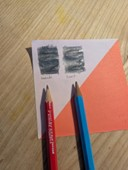
\includegraphics[height=0.3\textheight]{Bild1.jpg}
	\caption{Auftragen der Schichten mit verschiedenen Bleistiften}\label{fig:bild1}
\end{figure}
\newpage

\noindent Mit einem Multimeter\index{Multimeter} überprüften wir, wie gut die aufgetragene Schicht leitete und ob sie überhaupt leitfähig war. Der weichere Bleistift ermöglichte es, mehr Schichten aufzutragen, ohne dass das Papier riss, weshalb diese Schicht besser leitete.
\begin{figure}[htbp]
	\centering
	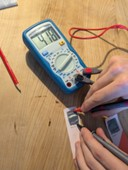
\includegraphics[height=0.3\textheight]{Bild2.jpg}
	\caption{Messung der Leitfähigkeit mit einem Multimeter}\label{fig:bild2}
\end{figure}

\vspace{12px}

\noindent Anschliessend befestigten wir je einen Draht mit Klebestreifen am Papier und verbanden ihn mit der Kohlenstoffschicht, indem wir leitende Farbe verwendeten.
\begin{figure}[htbp]
	\centering
	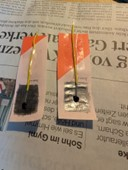
\includegraphics[height=0.3\textheight]{Bild3.jpg}
	\caption{Befestigung der Drähte mit Klebestreifen}\label{fig:bild3}
\end{figure}
\newpage

\noindent 
\sloppy 
Danach klebten wir ein Stück Aluminiumprofil\index{Aluminiumprofil}, das wir zuvor auf den grösseren Flächen leicht abgeschliffen hatten, auf das Papier und verbanden es mit einem Kabel.
\begin{figure}[htbp]
	\centering
	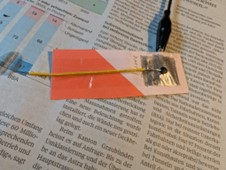
\includegraphics[height=0.3\textheight]{Bild4.jpg}
	\caption{Befestigung des Aluminiumprofils}\label{fig:bild4}
\end{figure}

\vspace{12px}

\noindent Als Elektrolyt\index{Elektrolyt} für unsere Batterie nutzten wir eine Kochsalzlösung\index{Kochsalzlösung}, in die wir die Batterie eintauchten, wobei wir darauf achteten, dass jeweils nur ein Kabel im Wasser war. Wie im Bild zu sehen ist, konnte die Batterie tatsächlich Spannung erzeugen.
\begin{figure}[htbp]
	\centering
	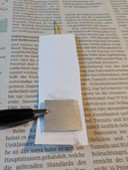
\includegraphics[height=0.3\textheight]{Bild5.jpg}
	\caption{Test der Bleistift-Schicht-Batterie in Kochsalzlösung\index{Kochsalzlösung}}\label{fig:bild5}
\end{figure}
\newpage

\noindent Dies hielt jedoch nicht lange an, da die Farbe wasserlöslich ist und sich das Papier wölbte, wodurch der Kontakt zum Aluminiumprofil beeinträchtigt wurde.
\begin{figure}[htbp]
	\centering
	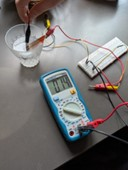
\includegraphics[height=0.3\textheight]{Bild6.jpg}
	\caption{Probleme mit der Leitfähigkeit aufgrund der Papierwölbung}\label{fig:bild6}
\end{figure}

\vspace{12px}

\begin{figure}[htbp]
	\centering
	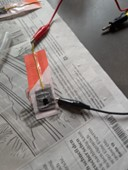
\includegraphics[height=0.3\textheight]{Bild7.jpg}
	\caption{Kurze Pause für die Batteriezelle}\label{fig:bild7}
\end{figure}

\newpage

\noindent Nach einer kurzen Pause versuchten wir es erneut, doch diesmal löste sich die Farbe komplett und der Kontakt ging verloren.
\begin{figure}[htbp]
	\centering
	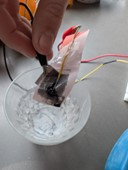
\includegraphics[height=0.3\textheight]{Bild8.jpg}
	\caption{Probleme mit der Leitfähigkeit aufgrund der Papierwölbung}\label{fig:bild8}
\end{figure}

\section{Versuch mit Graphit-Aluminium-Batterien}

\noindent Für die zweite Batterie haben wir zuerst eine Handvoll Bleistiftminen über einer Kerze ausgebrannt.
\begin{figure}[htbp]
	\centering
	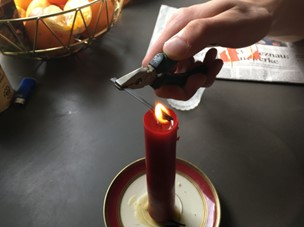
\includegraphics[height=0.3\textheight]{Bild9.jpg}
	\caption{Ausbrennen der Minen}\label{fig:bild9}
\end{figure}
\newpage

\noindent Diese haben wir anschliessend in Küchenpapier eingepackt und so in Aluminiumfolie gewickelt, dass die Minen keinen direkten Kontakt mit dem Aluminium haben.
\begin{figure}[htbp]
	\centering
	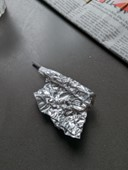
\includegraphics[height=0.3\textheight]{Bild10.jpg}
	\caption{In Küchenpapier und Aluminiumfolie eingewickelte Minen}\label{fig:bild10}
\end{figure}

\vspace{12px}

\noindent Die Zelle mit den ausgebrannt Minen hat deutlich besser funktioniert, mehr Spannung geliefert und auch wesentlich länger gehalten, da keine wasserlöslichen Stoffe enthalten waren. Als Elektrolyt\index{Elektrolyt} wurde erneut eine Kochsalzlösung\index{Kochsalzlösung} verwendet.
\begin{figure}[htbp]
	\centering
	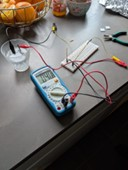
\includegraphics[height=0.3\textheight]{Bild11.jpg}
	\caption{Test der Graphit-Aluminium-Batterie in Kochsalzlösung\index{Kochsalzlösung}}\label{fig:bild11}
\end{figure}
\newpage

\noindent  
Wir haben nach dem gleichen Prinzip noch eine zweite Zelle mit nicht ausgebrannten Minen hergestellt. Diese hat jedoch deutlich weniger Spannung geliefert.
\begin{figure}[htbp]
	\centering
	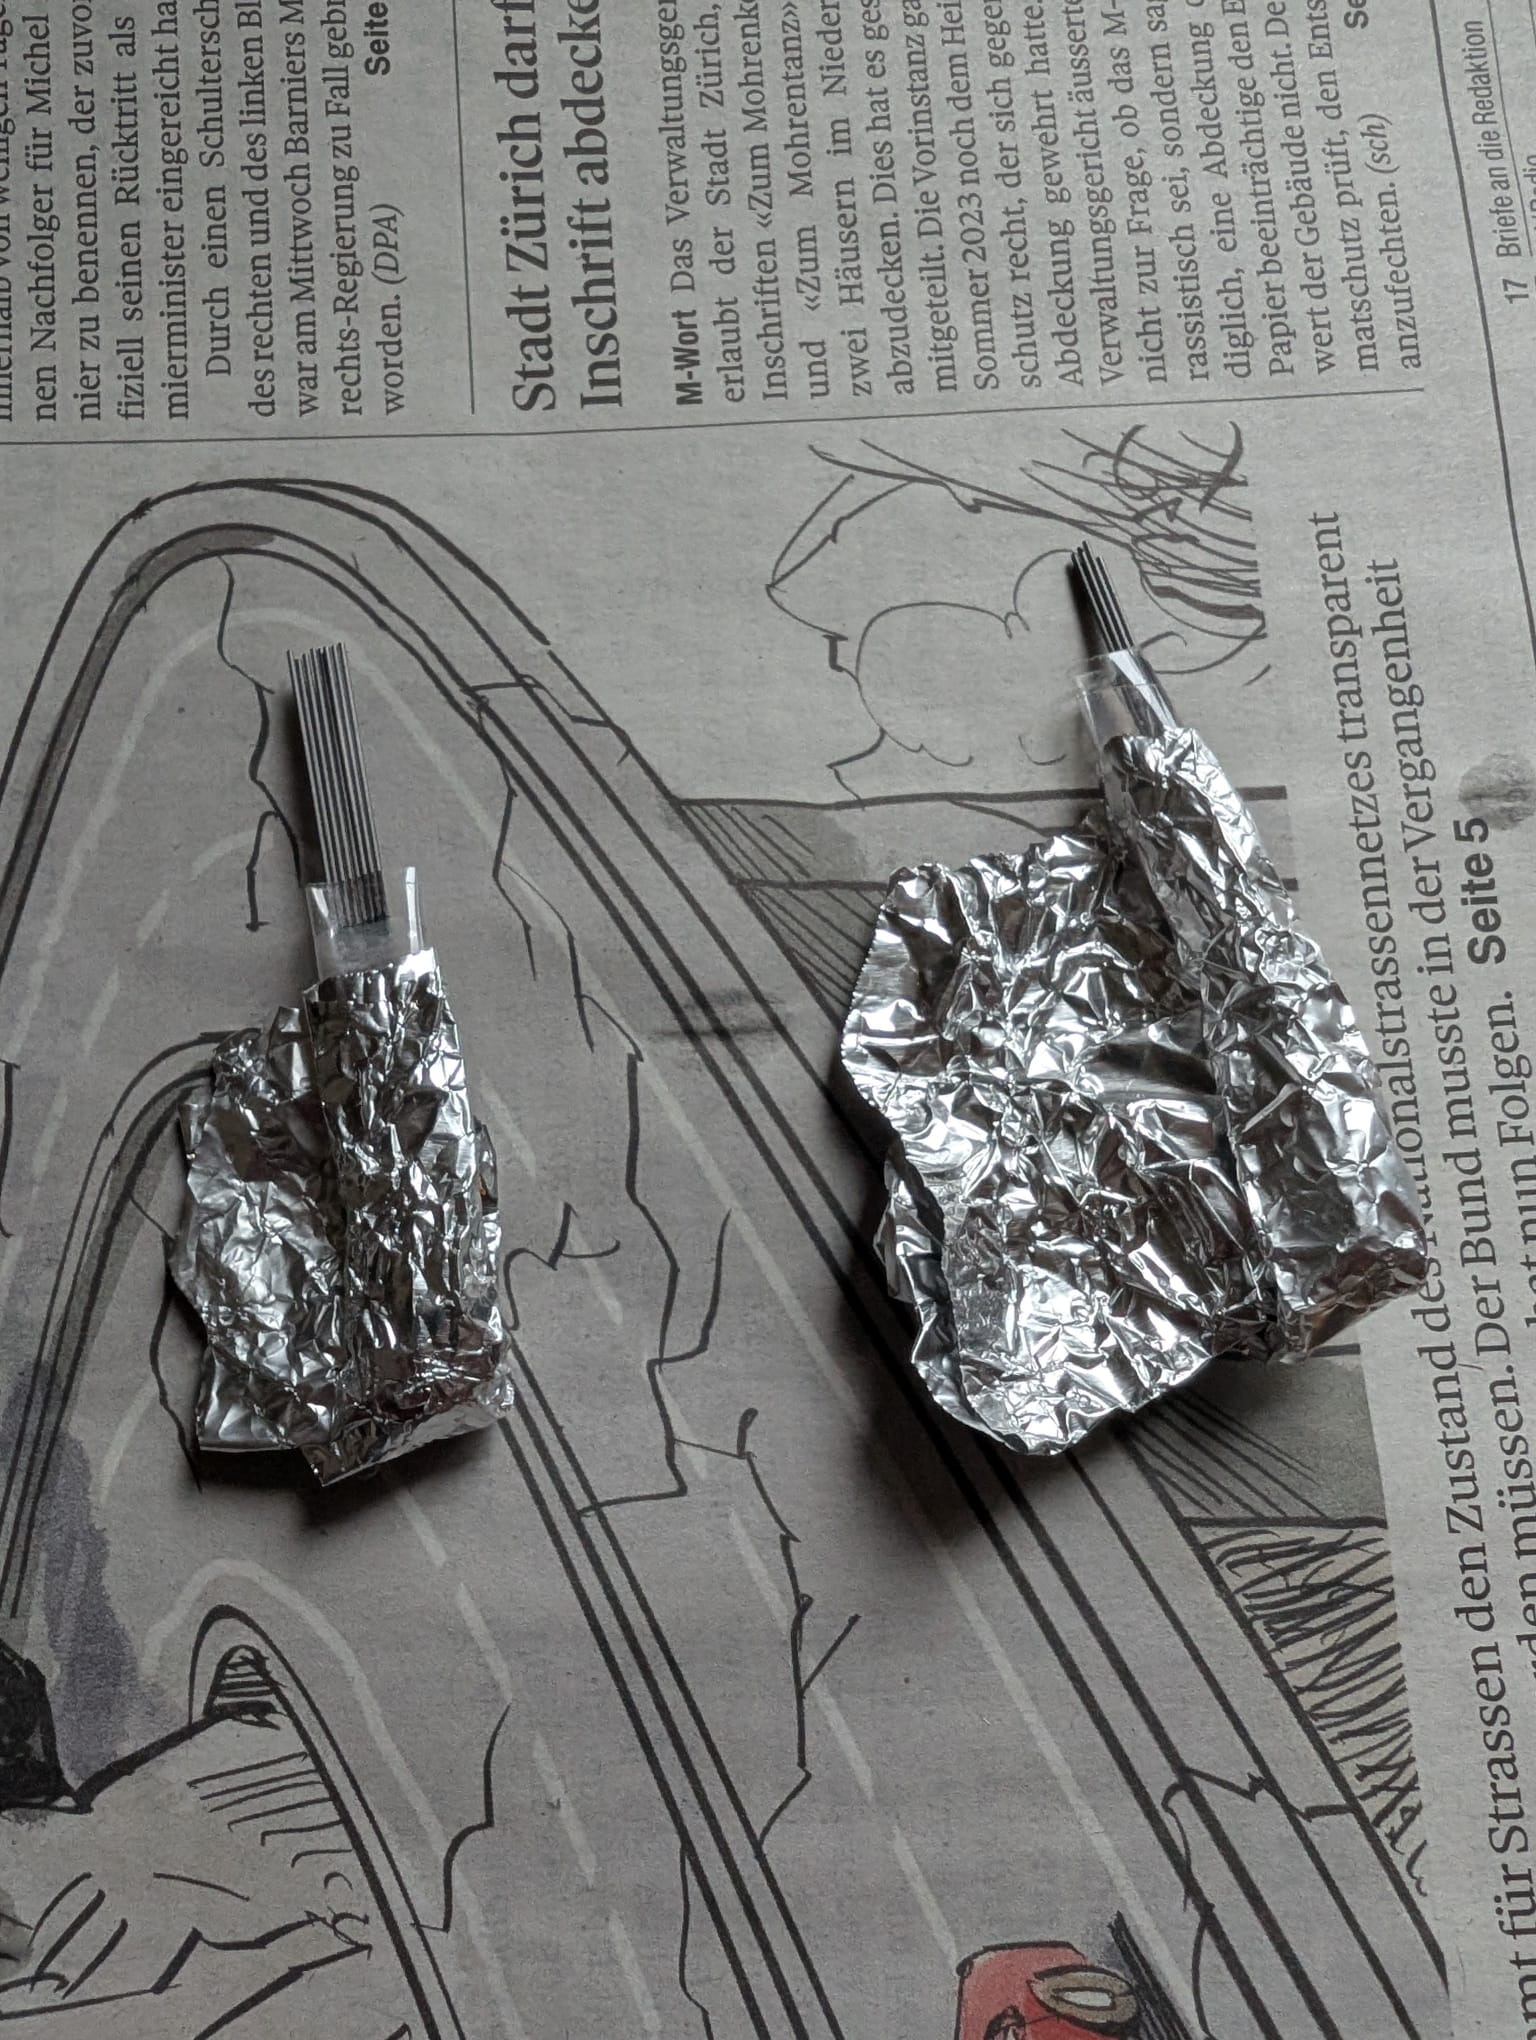
\includegraphics[height=0.3\textheight]{Bild12.jpg}
	\caption{Batterie mit nicht ausgebrannten Minen (links)}\label{fig:bild12}
\end{figure}

\vspace{12px}

\begin{figure}[htbp]
	\centering
	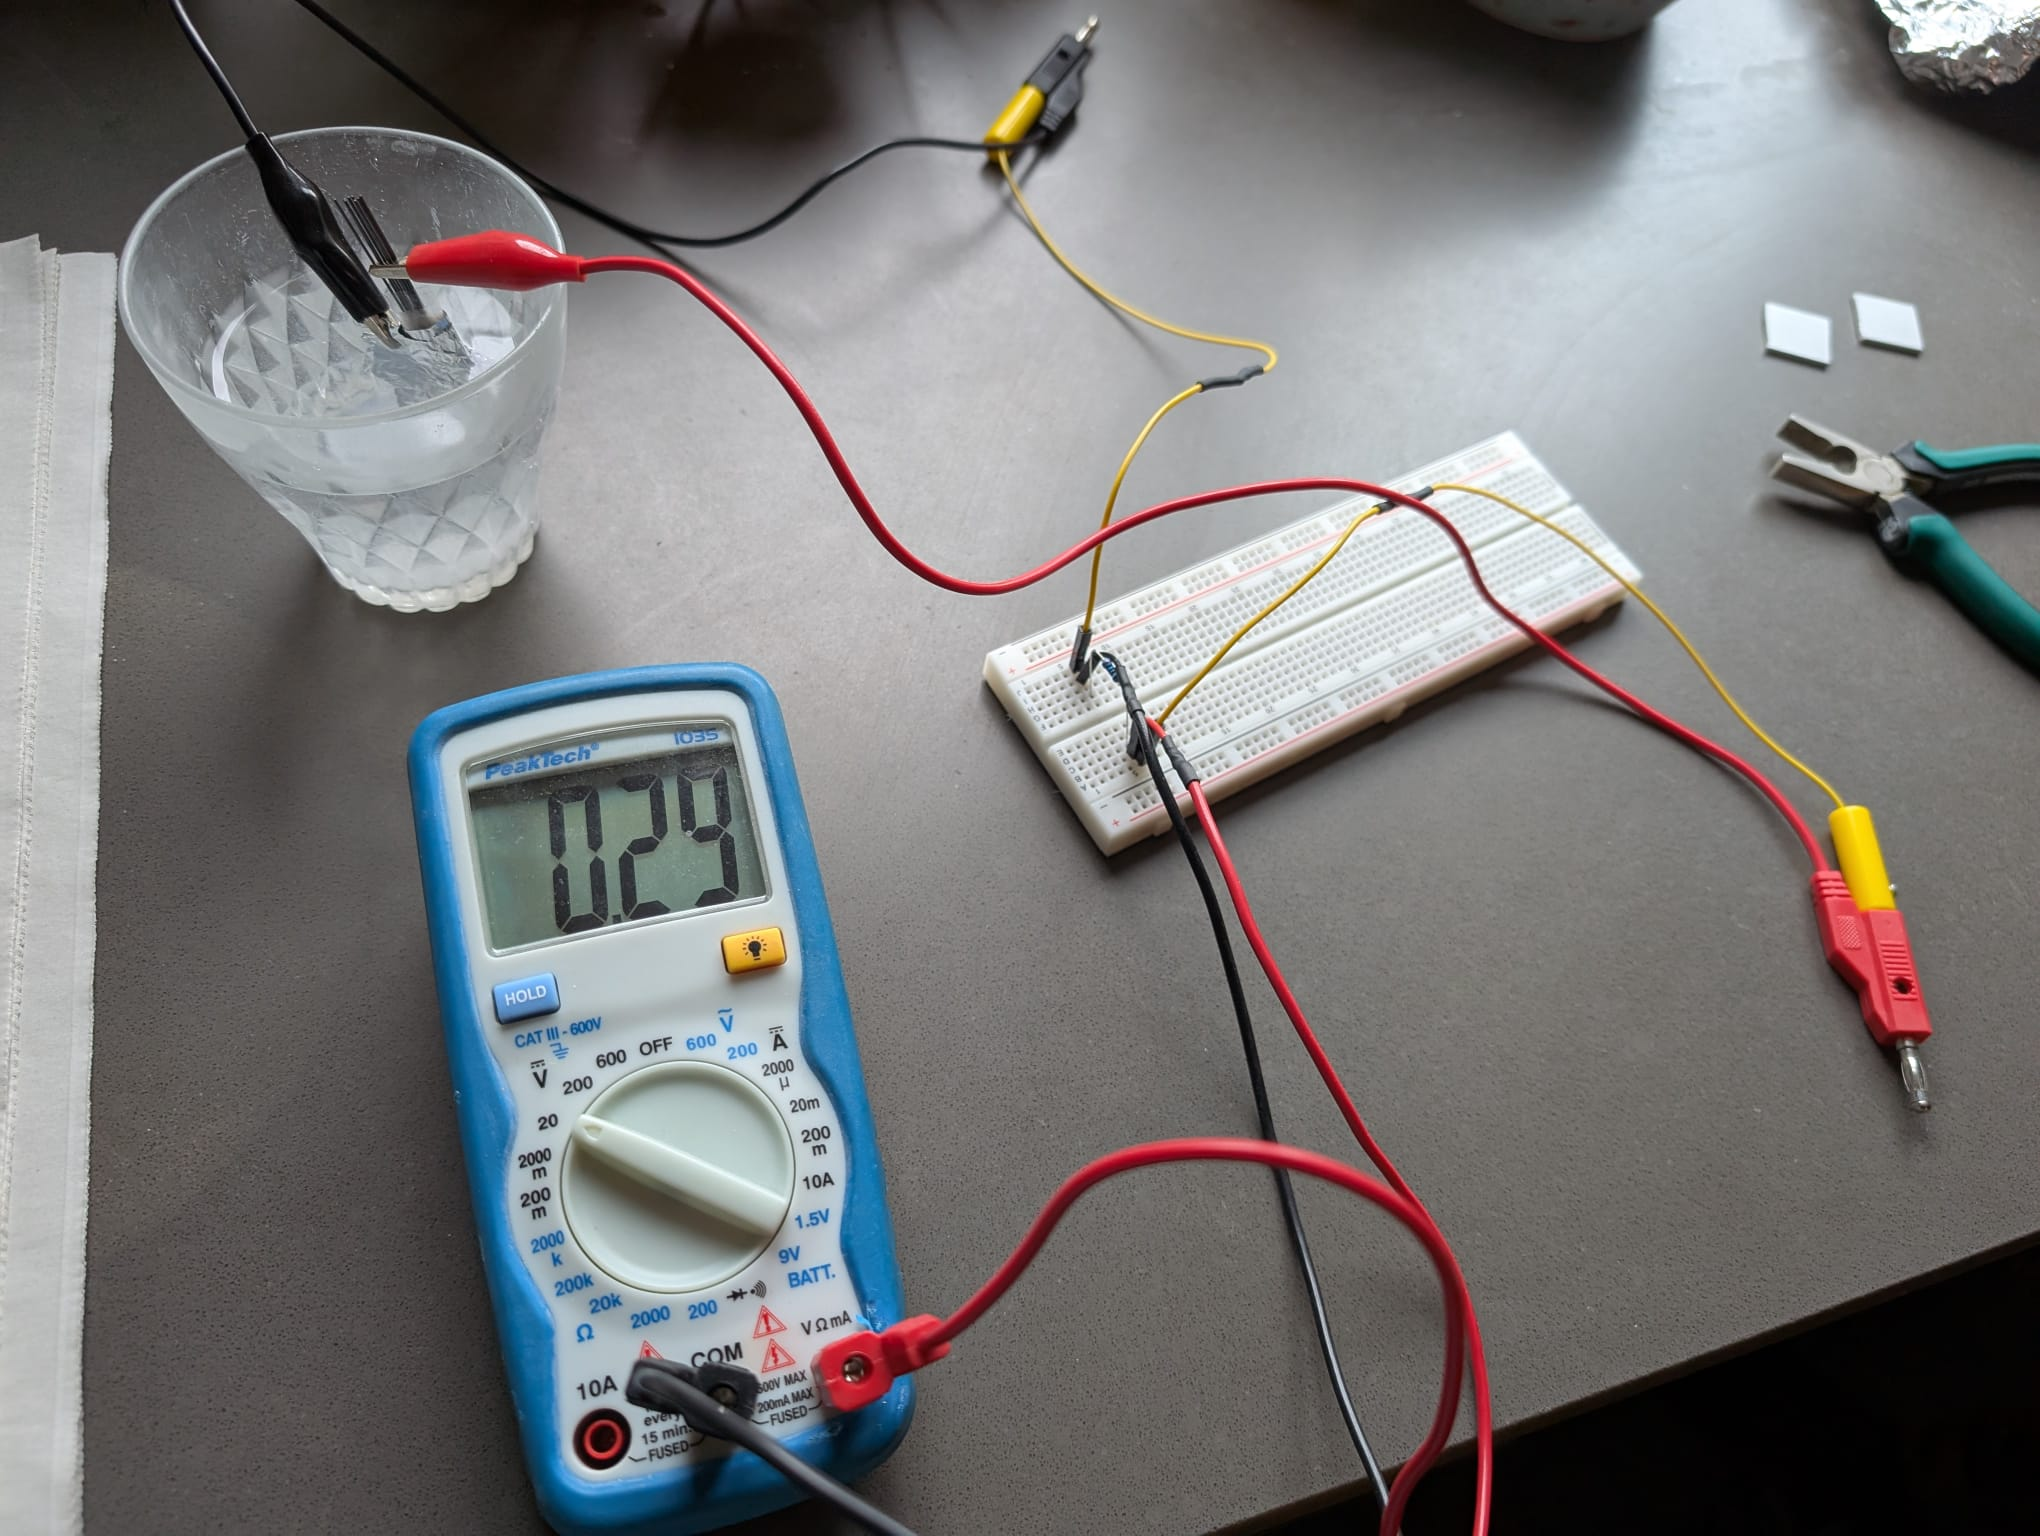
\includegraphics[height=0.3\textheight]{Bild13.jpg}
	\caption{Test der Batterie mit nicht ausgebrannten Minen}\label{fig:bild13}
\end{figure}
\newpage

\section{Erhöhung der Spannung durch Serieschaltung}

\noindent Als letztes wollten wir nun noch testen, wie gut man solche Zellen in Serie schalten kann. Dazu haben wir eine weitere Zelle mit ausgebrannten Minen hergestellt und die beiden Mittels einem dritten Kabel verbunden. Auf dem Bild kann man sehen, dass man so die Spannung tatsächlich erhöhen kann.
\begin{figure}[htbp]
	\centering
	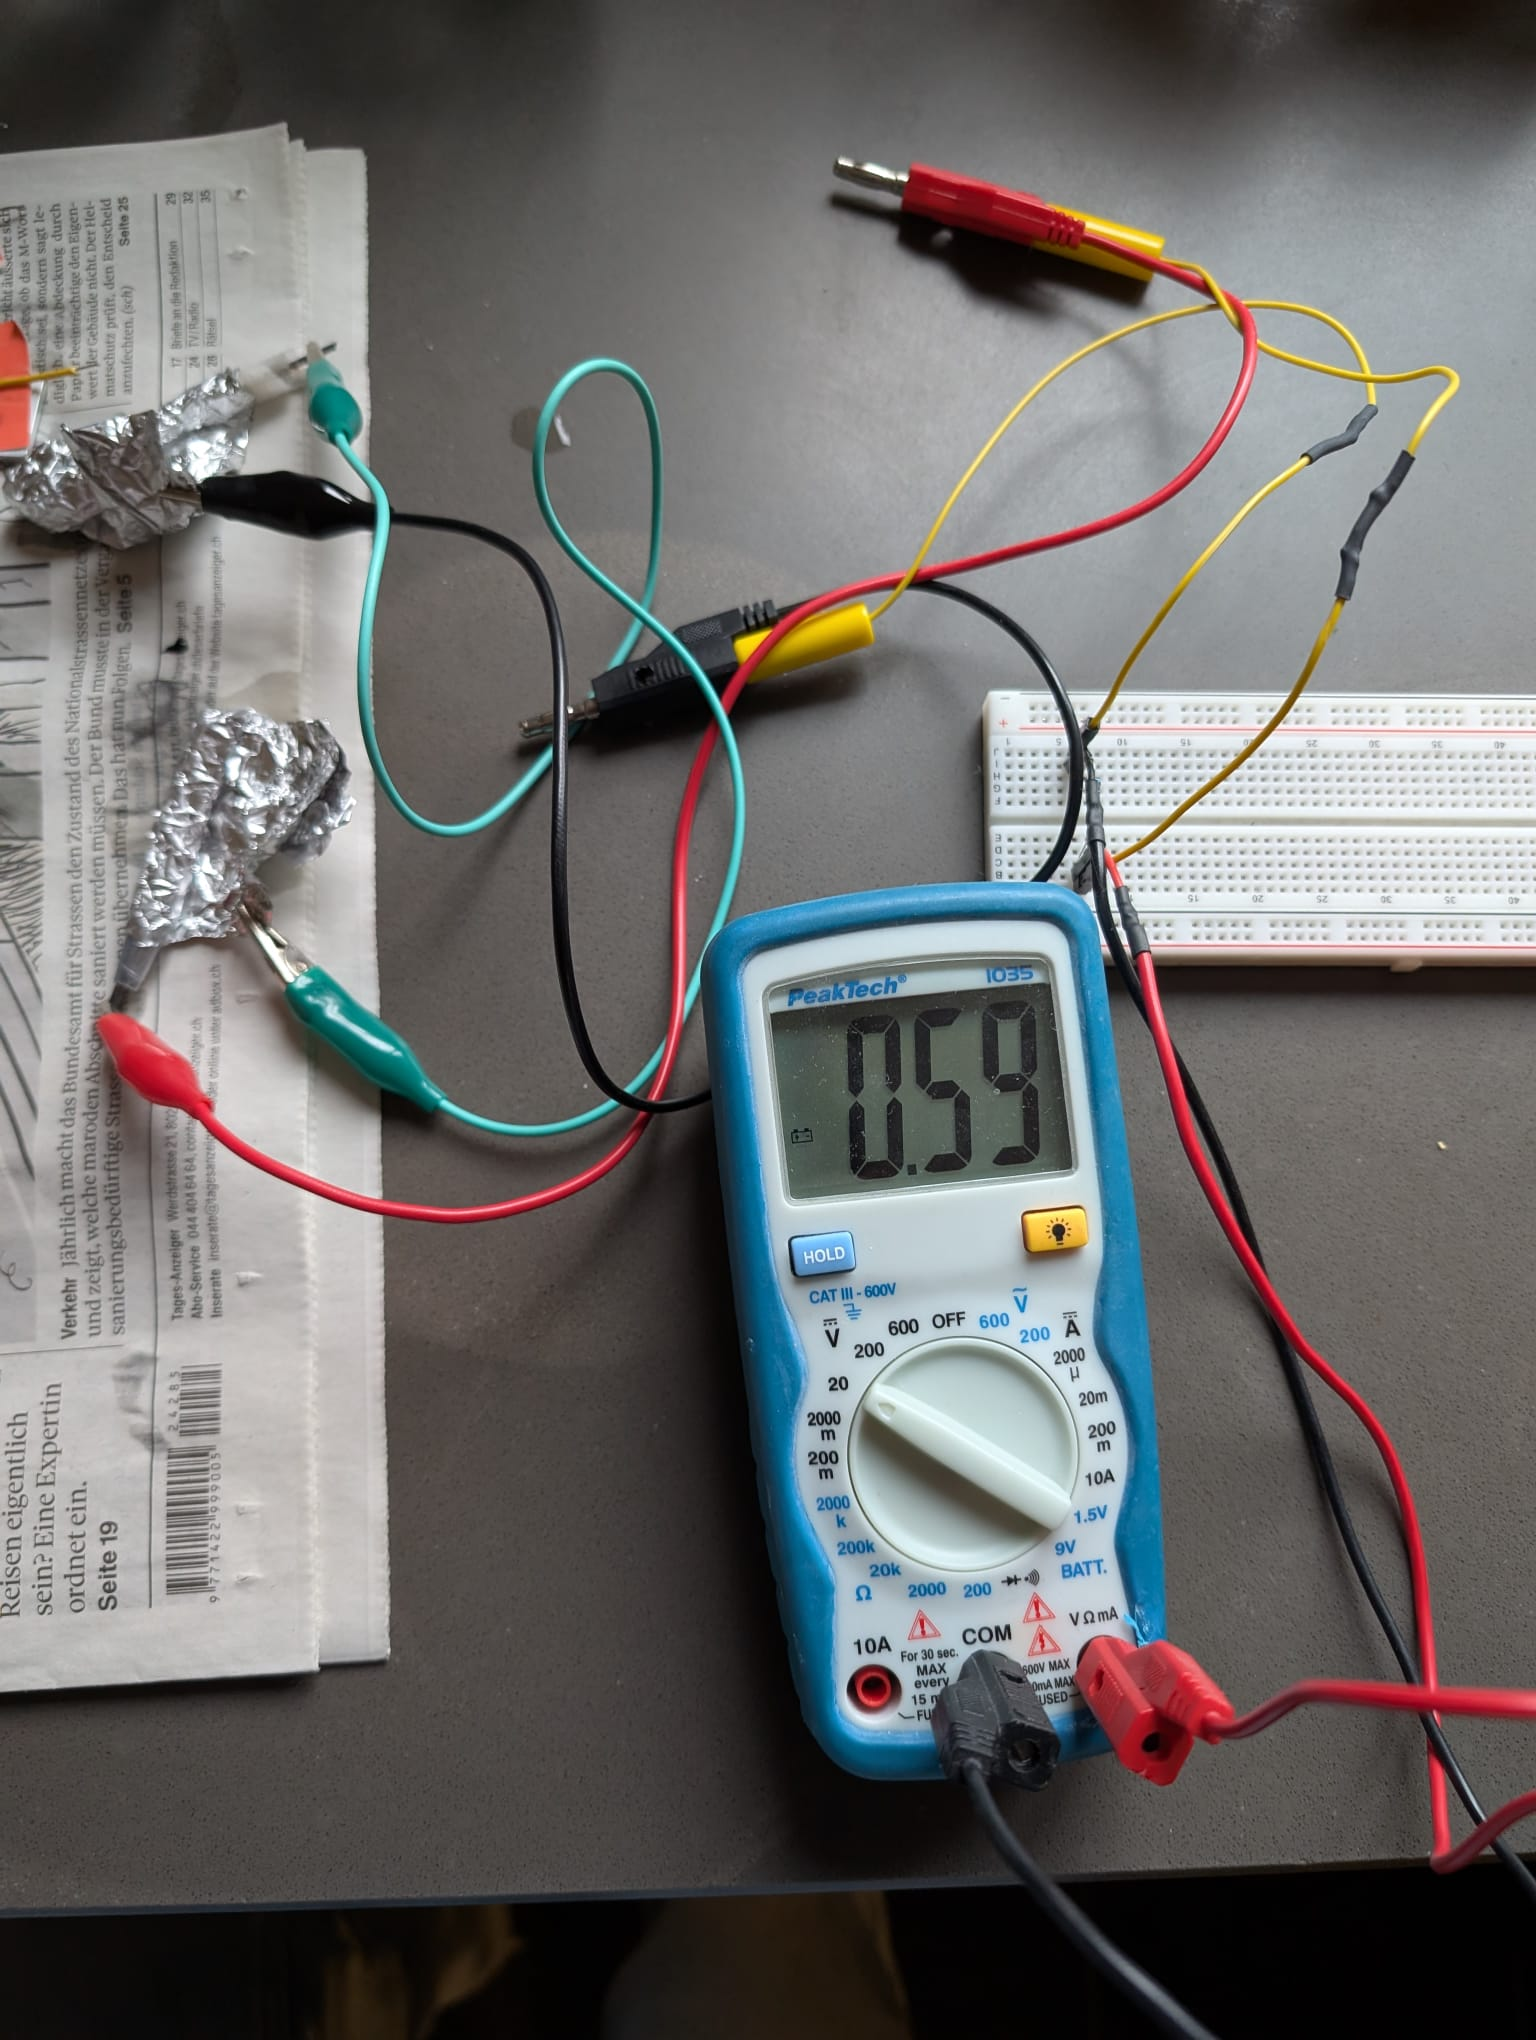
\includegraphics[height=0.3\textheight]{Bild14.jpg}
	\caption{Zwei Zellen in Serie geschalten}\label{fig:bild14}
\end{figure}

\vspace{12px}

\noindent Wenn das Papier sich einem vollgesaugt hat, funktioniert der Prozess auch ausserhalb der Gläser.
\begin{figure}[htbp]
	\centering
	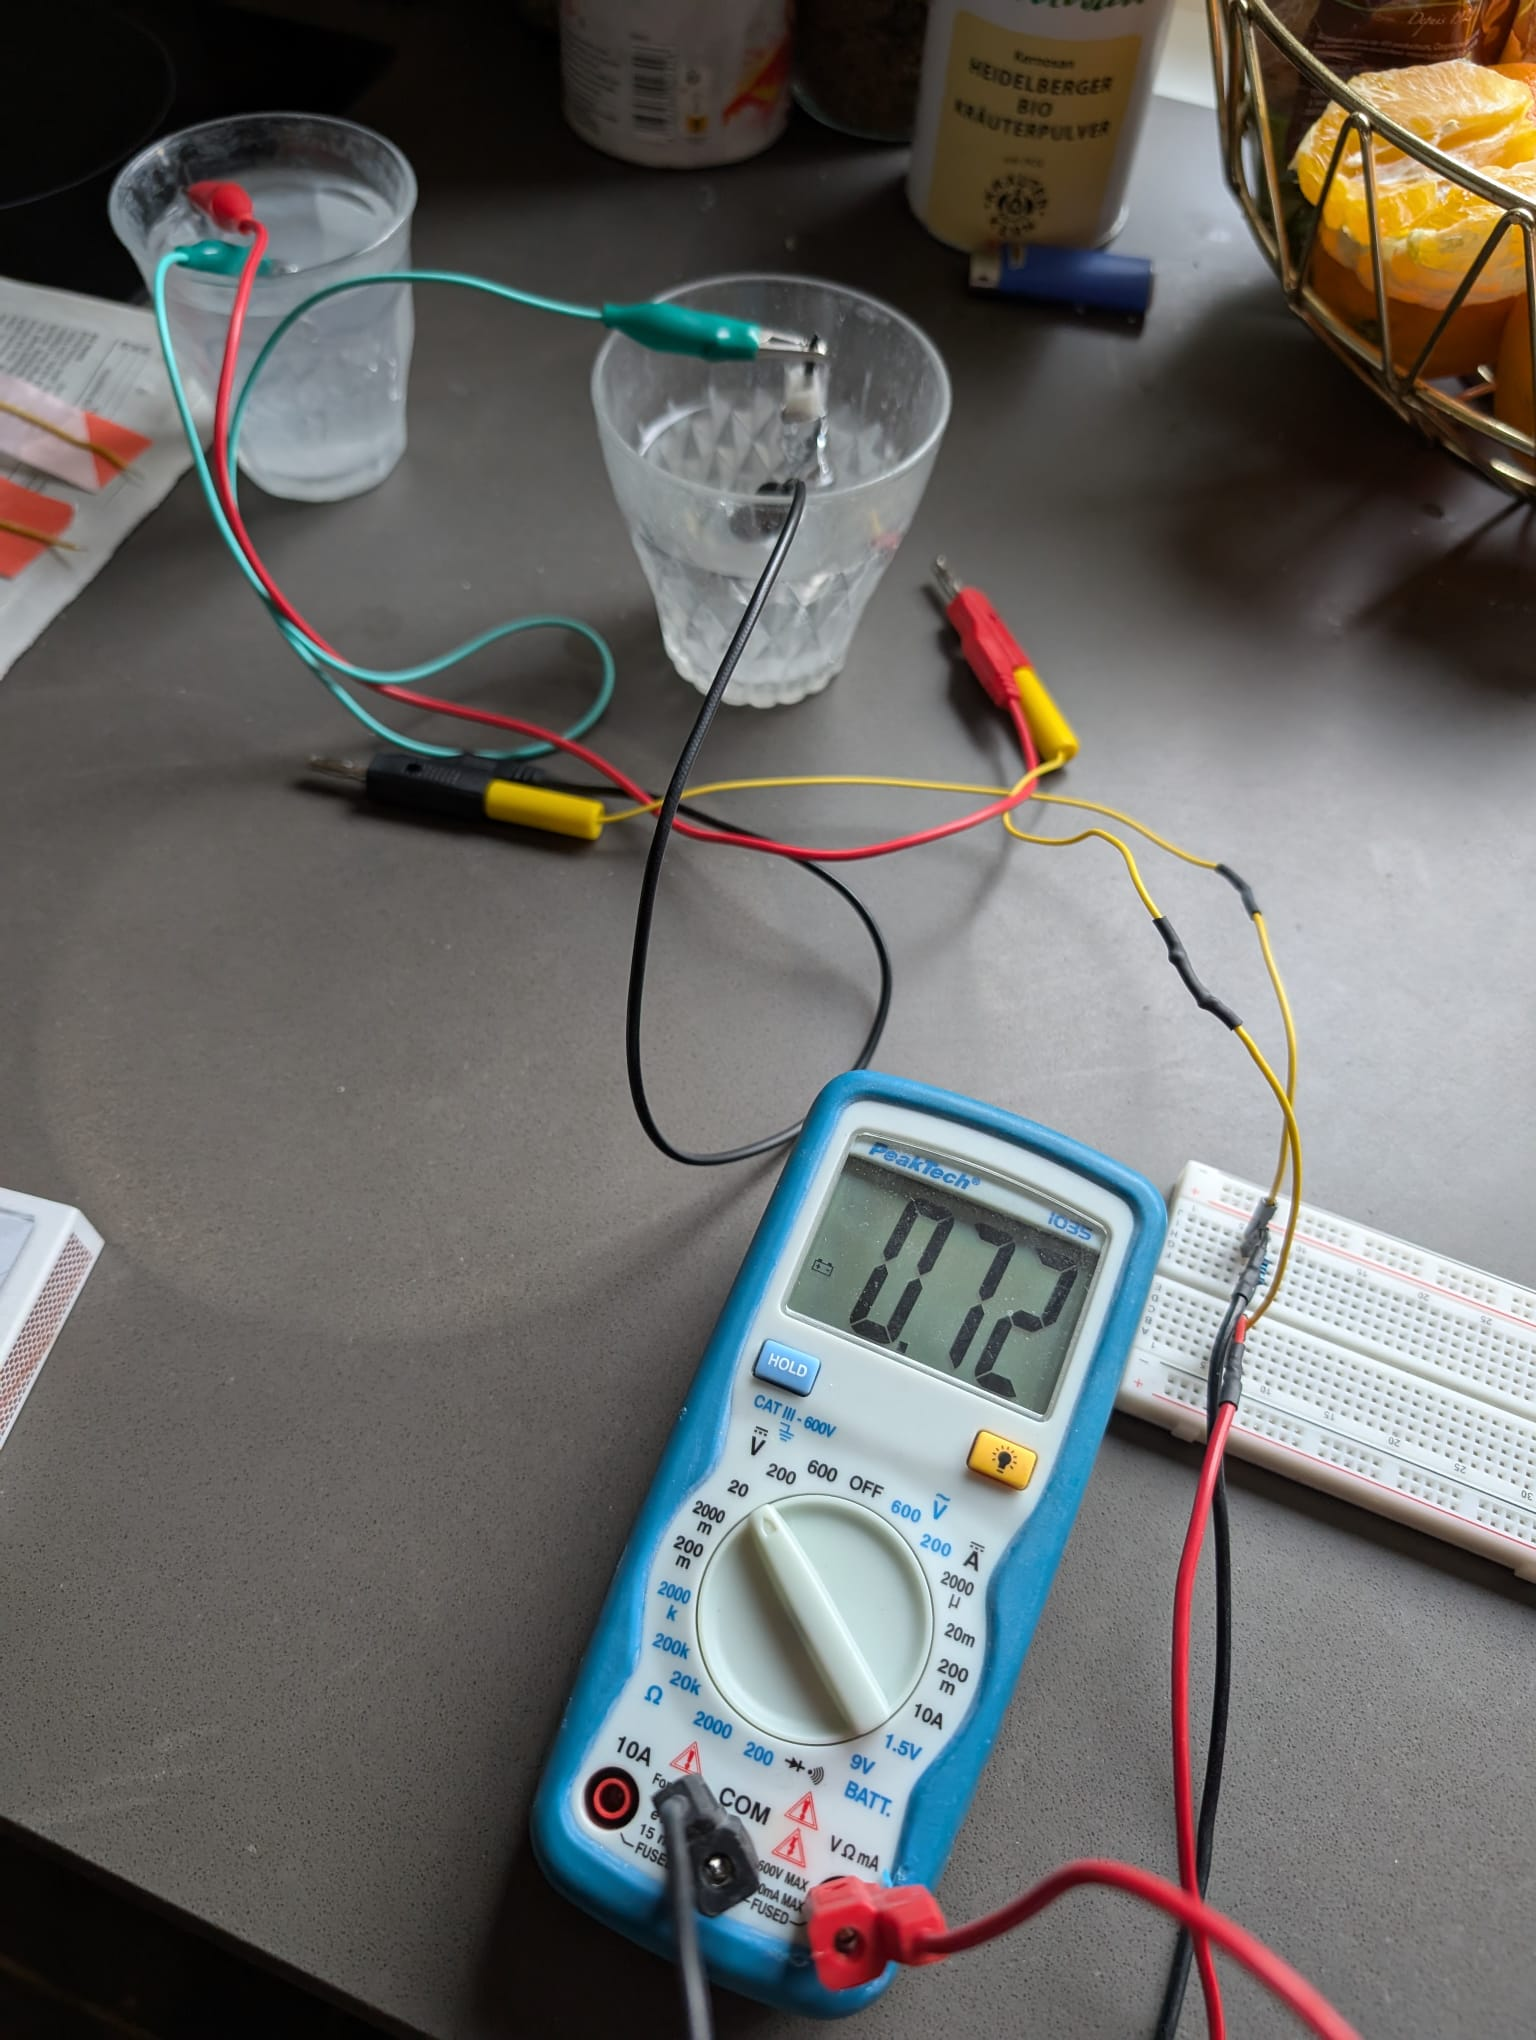
\includegraphics[height=0.3\textheight]{Bild15.jpg}
	\caption{Batteriezelle ausserhalb der Kochsalzlösung\index{Kochsalzlösung}}\label{fig:bild15}
\end{figure}
\newpage

\section{Funktionsweise einer Batterie}

Elektronen-Ionen-Batterien~\index{Elektronen-Ionen-Batterien}, wie in unserem Experiment mit Graphit-Aluminium-Batterien, nutzen die elektrochemische Reaktion zur Erzeugung von elektrischer Energie. Eine solche Batterie besteht aus zwei Elektroden, einem Elektrolyten\index{Elektrolyt} und einer elektrischen Verbindung, die den Strom von der Anode (negativ) zur Kathode (positiv) ermöglicht.


\subsection{Aufbau der Batterie}
Im Fall der Graphit-Aluminium-Batterie haben wir Graphit als Anode und Aluminium als Kathode verwendet. Als Elektrolyt\index{Elektrolyt} dient eine \textbf{Kochsalzlösung}\index{Kochsalzlösung}. Der chemische Prozess läuft folgendermassen ab:

\[
\text{Anode: } \text{Al} \rightarrow \text{Al}^{3+} + 3e^-
\]
\[
\text{Kathode: } 3\text{e}^- + 3\text{H}_2\text{O} \rightarrow \text{Al (OH)}_3
\]
Dabei gibt Aluminium \textit{Elektronen} ab, die über den externen Stromkreis zur Kathode fliessen und dort eine chemische Reaktion auslösen.\cite{author1}

\subsection{Elektronenfluss und Ionenbewegung}
Die Elektronen fliessen von der Anode durch den externen Stromkreis (in unserem Experiment über die \textcolor{blue}{Drähte} und das \textit{Aluminiumprofil}) zur Kathode. Gleichzeitig bewegen sich die Ionen im \textcolor{red}{Elektrolyten}\index{Elektrolyt} von der Anode zur Kathode, um die elektrochemische Reaktion zu vervollständigen.

\subsection{Spannungserzeugung}
Die Spannung einer Batterie wird durch die Differenz des elektrochemischen Potentials zwischen den Elektroden bestimmt.\cite{author3} In unserem Fall war es die Reaktion zwischen Aluminium und Graphit, die eine \textit{Spannung} erzeugte. Diese Spannung kann durch die Serien- oder Parallelschaltung mehrerer Zellen erhöht werden.

\begin{equation}
    V_{\text{gesamt}} = V_1 + V_2 + \cdots + V_n
    \label{eq:gesammtspannung}
\end{equation}
\noindent Dies~\eqref{eq:gesammtspannung} bedeutet, dass die Spannung jeder Zelle addiert wird, wenn sie in Serie geschaltet werden, was eine höhere Ausgangsspannung ermöglicht.

\subsection{Diagramm der Spannung über Zeit}\label{sec:tabelle}
Im Experiment messen wir die Spannung einer einzelnen Batterie über einen Zeitraum. Angenommen, wir haben die Spannung einer Zelle über 10 Minuten hinweg gemessen und die folgenden Daten aufgezeichnet:

\begin{table}[ht!]
\centering
\begin{tabular}{|c|c|}
\hline
\textbf{Zeit (min)} & \textbf{Spannung (V)} \\
\hline
0 & 0.79 \\
1 & 0.72 \\
2 & 0.65 \\
3 & 0.59 \\
4 & 0.54 \\
5 & 0.51 \\
6 & 0.48 \\
7 & 0.46 \\
8 & 0.44 \\
9 & 0.43 \\
10 & 0.43 \\
\hline
\end{tabular}
\caption{Spannungsabfall der Batterie über die Zeit}
\end{table}

\noindent Die Spannung nimmt kontinuierlich ab, da sich die chemischen Reaktionen im Inneren der Batterie mit der Zeit erschöpfen.\cite{author4}

\begin{figure}[ht!]
\centering
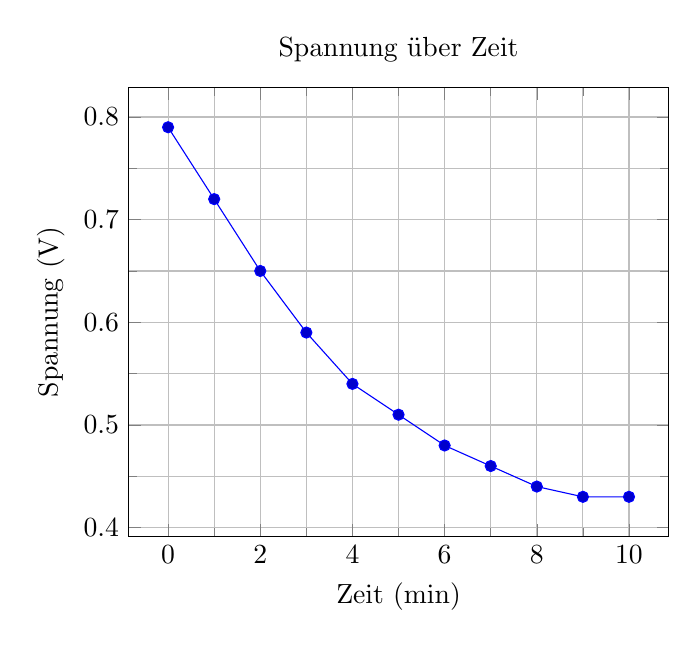
\begin{tikzpicture}
    \begin{axis}[
        title={Spannung über Zeit},
        xlabel={Zeit (min)},
        ylabel={Spannung (V)},
        grid=both,
        minor tick num=1,
        enlarge x limits={abs=0.5cm},
        enlarge y limits={abs=0.5cm},
    ]
    \addplot coordinates {
        (0,0.79)(1,0.72)(2,0.65)(3,0.59)(4,0.54)(5,0.51)(6,0.48)(7,0.46)(8,0.44)(9,0.43)(10,0.43)
    };
    \end{axis}
\end{tikzpicture}
\caption{Spannung der Batterie über 10 Minuten}
\end{figure}

\subsection{Fussnoten}
Die Reaktion innerhalb der Zelle führt zu einem ständigen Abbau der Reaktionsfähigkeit der Elektroden, was sich direkt auf die Spannung auswirkt. Dies ist ein typisches Verhalten bei elektrochemischen Zellen\footnote{Die elektrochemische Reaktion führt zum Abbau von Reaktionsmaterialien, wodurch die Zellspannung mit der Zeit sinkt.\cite{author2}}.

\newpage

\section{Schriftformatierungen}
\textbf{Fettdruck}, \\
\textit{Kursivdruck}, \\
\textcolor{blue}{blaue Schriftfarbe}, \\
\Large manuell angepasste Schriftgrösse, \\
\textsf{dieser Text in Helvetica.}

\section{Verweise}
Dieser Abschnitt enthält einen Verweis auf \hyperref[sec:tabelle]{Abschnitt~\ref*{sec:tabelle}} auf Seite~\pageref{sec:tabelle}.

\section{Externe Links}
Ein Link zu \href{https://www.latex-project.org}{LATEX-Projektseite}.

\section{QR-Code}
Ein QR-Code zur LATEX-Projektseite:
\qrcode{https://www.latex-project.org}

\newpage

\section{Codelisting}
Ein Beispielcode:
\begin{lstlisting}[language=Python, caption={Beispielcode in Python}]
def hello_world():
    print("Hello, world!")
\end{lstlisting}

\newpage
\bibliographystyle{plain}
\begin{thebibliography}{99}


\bibitem{author1} John Doe, \textit{Experimentelle Physik in der Batterietechnologie}, Wissenschaftsverlag , 2020.

\bibitem{author2} Jane Smith, \textit{Neue Entwicklungen in der Batterietechnologie}, Zeitschrift für Energietechnik, Vol. 42, No. 7, 2022, pp. 150-160.

\bibitem{author3} Max Mustermann, \textit{Batterie-Technologien: Vergangenheit, Gegenwart und Zukunft}, Springer Verlag, 2018.

\bibitem{author4} Lisa Meier, \textit{Die Rolle von Graphit in modernen Batterien}, Journal of Material Science, 2021.

\end{thebibliography}

\newpage
\printindex[columns=1, title=Index]

\end{document}
